\documentclass[12pt,twoside,a4paper,polish]{report}
\usepackage[T1]{fontenc}
\usepackage{babel}

\usepackage[utf8]{inputenc} % https://tex.stackexchange.com/a/44699

% \usepackage{indentfirst}

\renewcommand{\thechapter}{\arabic{chapter}.}
\renewcommand{\thesection}{\thechapter\arabic{section}.}
\renewcommand{\thesubsection}{\thesection\arabic{subsection}.}

\setlength\parindent{1.25cm}

\usepackage[vmargin=2.5cm,lmargin=3cm,rmargin=2.5cm,includehead]{geometry}

\usepackage{fancyhdr}
\pagestyle{fancy}
\fancyhf{}
\fancyheadoffset{0cm}
\renewcommand{\headrulewidth}{0pt}
\renewcommand{\footrulewidth}{0pt}
\fancyhead[LO,RE]{\thepage}
\fancypagestyle{plain}{\fancyhf{}\fancyhead[LO,RE]{\thepage}}

\setlength{\headheight}{14.49998pt} % https://tex.stackexchange.com/a/327298

\usepackage{helvet}
\renewcommand{\familydefault}{\sfdefault}

\linespread{1.5}

% https://texfaq.org/FAQ-run-fn-nos
\usepackage{chngcntr}
\counterwithout*{footnote}{chapter}

% https://tex.stackexchange.com/a/28334
\usepackage{chngcntr}
\counterwithout*{figure}{chapter}

% \renewcommand{\theequation}{\arabic{equation}}

\usepackage{graphicx}
\usepackage[export]{adjustbox} % Used to occasionally get the frame around the graphic.

\usepackage[tablename=Tab.,figurename=Rys.,labelsep=space]{caption} % https://tex.stackexchange.com/a/287616 & https://tex.stackexchange.com/a/192451
\newcommand{\source}[1]{\caption*{\footnotesize{Źródło: {#1}}}} % https://tex.stackexchange.com/a/246285
\renewcommand{\thetable}{\arabic{table}.}
\renewcommand{\thefigure}{\arabic{figure}.}

\usepackage[algoruled]{algorithm2e}
\SetAlgorithmName{Algorytm}{Spis algorytmów}{Spis algorytmów}

\usepackage{listings}

\lstset{
    literate=
        {ą}{{\k{a}}}1
        {Ą}{{\k{A}}}1
        {ć}{{\'{c}}}1
        {Ć}{{\'{C}}}1
        {ę}{{\k{e}}}1
        {Ę}{{\k{E}}}1
        {ł}{{\l{}}}1
        {Ł}{{\l{}}}1
        {ń}{{\'{n}}}1
        {Ń}{{\'{N}}}1
        {ó}{{\'{o}}}1
        {Ó}{{\'{O}}}1
        {ś}{{\'{s}}}1
        {Ś}{{\'{S}}}1
        {ż}{{\.{z}}}1
        {Ż}{{\.{Z}}}1
        {ź}{{\'{z}}}1
        {Ź}{{\'{Z}}}1
} % https://stackoverflow.com/a/52434857

\renewcommand{\lstlistlistingname}{Spis implementacji} % https://sunsite.icm.edu.pl/pub/CTAN/macros/latex/contrib/listings/listings.pdf (35) & https://stackoverflow.com/a/9480618

\renewcommand{\lstlistingname}{Implementacja} % https://sunsite.icm.edu.pl/pub/CTAN/macros/latex/contrib/listings/listings.pdf (36)

\lstset{numberbychapter=false} % https://sunsite.icm.edu.pl/pub/CTAN/macros/latex/contrib/listings/listings.pdf (36)

\lstset{basicstyle=\footnotesize,captionpos=b,frame=single,numbers=left} % https://en.wikibooks.org/wiki/LaTeX/Source_Code_Listings#Settings

\lstdefinelanguage{Go}{ % Based on https://github.com/korfuri/golang-latex-listings
  % Keywords as defined in the language grammar
  morekeywords=[1]{break,default,func,interface,select,case,defer,go,map,struct,chan,else,goto,package,switch,const,fallthrough,if,range,type,continue,for,import,return,var},
  % Built-in functions
  morekeywords=[2]{append,cap,close,complex,copy,delete,imag,len,make,new,panic,print,println,real,recover},
  % Pre-declared types
  morekeywords=[3]{bool,byte,complex64,complex128,error,float32,float64,int,int8,int16,int32,int64,rune,string,uint,uint8,uint16,uint32,uint64,uintptr},
  % Constants and zero value
  morekeywords=[4]{true,false,iota,nil},
  % Strings: "foo", 'bar', `baz`
  morestring=[b]{"},
  morestring=[b]{'},
  morestring=[b]{`},
  % Comments: /* comment */ and // comment
  comment=[l]{//},
  morecomment=[s]{/*}{*/},
  % Options
  sensitive=true
}

\usepackage{amsmath}

\title{Web browsers and Internet-connected devices digital fingerprinting methods - challenges and solutions}
\author{Artur Wolff}
\date{February 2021}

\usepackage[autostyle]{csquotes}  % TODO move 49-53 somewhere else;
\DeclareQuoteAlias{dutch}{polish} % https://tex.stackexchange.com/a/281280

\usepackage{biblatex}
\addbibresource{bib/references.bib}

\usepackage{pdfpages}

\begin{document}
\renewcommand{\thelstlisting}{\arabic{lstlisting}.} % It must be here because https://tex.stackexchange.com/a/49450

\includepdf{title/title}
% Uh... This is very bad, but it's better to do this here than in WYSIWYG.
\chapter*{Oświadczenie}

\section*{}
Wyrażam zgodę na udostępnianie mojej pracy w~czytelni Archiwum WAT.

\subsection*{}
Dnia \dotfill

\section*{}
\begin{flushright}
	Pracę przyjąłem
	\linebreak
	\linebreak
	\linebreak
	\linebreak
	promotor pracy\\
	ppłk dr inż. Rafał Kasprzyk
\end{flushright}

\tableofcontents
\chapter*{Wstęp}
% Zadania do pracy od promotora:
% 1. Podstawy funkcjonowania internetu - założenia i ich realizacja
% 2. Problematyka prywatności i anonimowości w internecie
% 3. Przegląd metod cyfrowego odcisku palca przeglądarek internetowych i urządzeń podłączonych do internetu
% 4. Wyzwania i rozwiązania związane z metodami cyfrowego odcisku palca
% 5. Opracowanie autorskich przykładów prezentujących możliwości metod cyfrowego odcisku palca
% 6. Przeprowadzenie eksperymentów i opracowanie wyników

\chapter*{Wstęp}

\chapter{Wprowadzenie do fingerprintingu}

\section{Podstawowe pojęcia}

\subsection{Nomenklatura używana w tej pracy}
Pisząc o odcisku palca, użyto (także w tytule pracy) ogólnie przyjętego skrótu
myślowego oznaczającego odbitkę linii papilarnych, czyli formę językową uznawaną
za poprawną przez specjalistów od daktyloskopii.

Użycie formy językowej ,,odcisk palca'' w terminie ,,cyfrowy odcisk palca'' ma
wiele sensu. Jeszcze bez zdefiniowania tego specjalistycznego terminu możemy
domyślić się, co oznacza. Oczywiście wynika to z faktu, że cyfrowy odcisk palca
i analogowy odcisk palca są ze sobą w pewien sposób powiązane (koncepcja
cyfrowego odcisku palca czerpie z wartości wynikających ze stosowania odbitek
ludzkich linii papilarnych w dziedzinie kryminalistyki).

Angielskie słowo ,,fingerprint'' tłumaczy się jako odcisk palca, jednakże w
zagranicznych publikacjach dotyczących cyfrowego odcisku palca rzadko występuje
termin ,,digital fingerprint''. Jak piszą Flood i Karlsson
\cite[s. 4]{flood2012browser}, kontekst użycia jest na tyle wyraźny, że użycie
samego ,,fingerprint'' jest wyczerpujące.

Zachodnie nazewnictwo ma tę przewagę, że jest zdecydowanie bardziej kompaktowe.
Także w przypadku słowotwórczego zabiegu \emph{fingerprinting} oznaczającego
czynność; szukając polskiego odpowiednika, musielibyśmy sięgnąć po ,,cyfrowe
znakowanie''. Z uwagi na tę kompaktowość i łatwość użycia w pracy preferowane
będzie użycie oryginalnej nomenklatury.

\subsection{Definicje}
W kolejnych punktach zawarto najważniejsze definicje i powiązane pojęcia
analogiczne do tych obecnych w literaturze
\cite{eckersley2010unique,flood2012browser}, które będą używane w przeciągu
całej pracy.

\subsubsection{Fingerprint}
Wektor cech pozwalający zidentyfikować dowolny zbiór danych.

Aby \emph{fingerprint} pełnił praktyczną funkcję identyfikacyjną tak jak odbitka
ludzkich linii papilarnych pełni praktyczną funkcję identyfikacyjną, często
stosuje się algorytm, który kojarzy wektor cech z określonej długości (zwykle
krótkim) ciągiem bajtów (identyfikatorem; można go także rozumieć jako
etykieta). Takim algorytmem może być na przykład wysokiej wydajności funkcja
skrótu (niekoniecznie zdatna do zastosowań kryptograficznych---na przykład
MurmurHash). W niektórych źródłach można także spotkać się z taką definicją, że
\emph{fingerprint} to już sam wynik wyżej wspomnianego algorytmu
\cite[s. 123--132]{wu2018beauty}. Taka definicja nie zmienia istoty
\emph{fingerprintu}, ale jest zdecydowanie mniej przydatna w kontekście
\emph{fingerprintingu} urządzeń podłączonych do Internetu i przeglądarek
internetowych.

\subsubsection{Fingerprint urządzenia podłączonego do Internetu}
Wektor cech pozwalający zidentyfikować urządzenie podłączone do Internetu.

\subsubsection{Instalacja przeglądarki internetowej}
Instalacja na konkretnym urządzeniu. W przypadku zmiany ustawień, konfiguracji i
liczby \emph{pluginów}/rozszerzeń oraz aktualizacji przeglądarki instalacja
przeglądarki pozostaje ciągle tą samą instalacją.

\subsubsection{Fingerprint przeglądarki internetowej}
Wektor cech pozwalający zidentyfikować instalację przeglądarki internetowej.

\subsection{Właściwości fingerprintu}
Ludzkie linie papilarne są na ogół niepowtarzalne, niezmienne i nieusuwalne. Z
wartości wynikających ze stosowania ich odbitek w swojej dziedzinie badawczej
czerpie (także etymologicznie) koncepcja \emph{fingerprintu} i dlatego też
\emph{fingerprint} z dobrze dobranymi cechami będzie odzwierciedlać podobne
właściwości.

W przypadku \emph{fingerprintu} urządzeń podłączonych do Internetu i
przeglądarek internetowych najważniejszymi jego właściwościami są unikalność /
różnorodność (niepowtarzalność) oraz stabilność (niezmienność), przy czym
zwiększenie unikalności lub stabilności ma najczęściej negatywny wpływ na drugi
parametr \cite[s. 11]{eckersley2010unique}.

Jedną ze stosowanych metod pomiaru unikalności \emph{fingerprintu} urządzeń i
przeglądarek jest entropia Shannona \cite[s. 6]{eckersley2010unique}.

\subsubsection{Entropia Shannona}
Wartość entropii można rozumieć jako liczbę pytań binarnych potrzebnych do
sklasyfikowania losowo wybranego elementu z danego zbioru. Zatem entropia
Shannona zbioru \(D\) z etykietami \(\{l_{0}, l_{1}, \dots, l_{n - 1}\}\) wyraża
się wzorem \[H(D) = -{\sum_{i = 0}^{n - 1}{p(l_{i})\log_{2}{p(l_{i})}}}\] gdzie
\(p(l_{i})\) to wyrażona ułamkiem częstość \(x \in D\) mającego etykietę
\(l_{i}\). W przypadku, w którym każda etykieta występuje tak samo często,
entropia ma wartość maksymalną równą \(\log_{2}{n}\).

\paragraph{Przykład}
Jeśli zbiór \emph{fingerprintów} przeglądarek internetowych ma \(32\) bity
entropii to w przypadku losowego wyboru jednego z nich oczekujemy, że w
najlepszym przypadku tylko \(1\) na \(4294967295\) przeglądarek będzie miała
taki sam \emph{fingerprint}.

\subsubsection{Stabilność}
W przypadku dodania kolejnej cechy do wektora cech identyfikującego urządzenie
lub przeglądarkę zwykle zwiększy to entropię, ale także zmniejszy stabilność
\emph{fingerprintu}. Dzieje się tak, ponieważ jest to kolejna rzecz, która może
zmienić się w czasie. Jeśli jedną z cech wejściowych jest wersja oprogramowania
urządzenia lub wersja przeglądarki (która zwykle zmienia się parę razy w ciągu
roku) to kolejne \emph{fingerprinty} mogą odbiegać od siebie i naiwny
klasyfikator korzystający z algorytmu reagującego na najmniejsze zmiany (na
przykład funkcja skrótu) mógłby nadać takiemu urządzeniu/przeglądarce kolejną
etykietę zamiast potraktowania jej jako poprzednio widzianą instalację.

\section{Fingerprinting a Internet} % https://sjp.pwn.pl/poradnia/haslo/;228
Aby lepiej zrozumieć istotę \emph{fingerprintu} i motywację stojącą za
stosowaniem \emph{fingerprintingu} w kontekście urządzeń podłączonych do
Internetu oraz przeglądarek internetowych wspominając o różnych innych obszarach
przetwarzania komputerowego, w których wykorzystywany jest \emph{fingerprinting}
w stosownych mu celach, kolejne punkty posłużą jako referencja (także
historyczna).

\subsection{Początki Internetu}
Początek Internetu, jaki znamy obecnie to początek stworzonej w 1969 roku na
potrzeby amerykańskiego wojska sieci ARPAnet. ARPAnet była implementacją
niezależnych prac Paula Barana, Donalda Daviesa i Leonarda Kleinrocka z lat 60.
XX wieku. Na samym początku swojego istnienia Internet wykorzystywany był do
tego, aby rozpraszać obliczenia pomiędzy wiele komputerów---w tym wypadku
chodziło o superkomputery znajdujące się w innych ośrodkach badawczych (ARPAnet
powstało na Uniwersytecie Kalifornijskim w Los Angeles) \cite{press2015very}. W
tym samym okresie powstawały inne globalne sieci komputerowe zapoczątkowane
zwykle w innym celu (na przykład komunikacyjnym, rozrywkowym), które później
połączono z ARPAnet. Badacze historii Internetu wskazują na fakt, iż gwałtowny
rozwój Internetu zawdzięcza się właśnie komunikacyjnemu i rozrywkowemu aspektowi
konkurencyjnych sieci \cite{maigret2012socjologia}.

\subsection{Założenia funkcjonowania Internetu i ich realizacja}
Po tym, jak w 1989 Tim Berners-Lee oraz Robert Cailliau utworzyli projekt sieci
dokumentów hipertekstowych, czyli tego, co obecnie znamy jako World Wide Web i
strony internetowe, osoby prywatne oraz instytucje komercyjne zaczęły dostrzegać
korzyści z użytkowania Internetu, a szczególnie z wykorzystania go jako medium
reklamy i sprzedaży \cite{press2015very}. Zniesienie zakazu wykorzystywania
Internetu do celów zarobkowych w 1991 roku zakończyło chwilę, w której Internet
był medium naukowego dyskursu i zapoczątkowało okres istnienia Internetu dla
mas, który trwa do dziś.

\subsubsection{Perspektywa techniczna}
Podstawą struktury obecnego Internetu jest model TCP/IP i koncepcyjnie składa
się ze współpracujących ze sobą 4 warstw \cite{kahn1974protocol}:
\begin{enumerate}
	\item dostępu do sieci
	\item kontroli transportu
	\item Internetu
	\item aplikacji
\end{enumerate}
W najwyższej z warstw, czyli warstwie aplikacji działają takie usługi jak
przeglądarka czy serwer WWW. To najbardziej interesująca warstwa z perspektywy
niniejszej pracy, ale \emph{fingerprinting} urządzeń podłączonych do Internetu
może odbywać się także w niższych warstwach. % TODO Elaborate?

\subsection{Początki śledzenia użytkowników Internetu}
Gwałtowny rozwój komercyjnego Internetu sprawił, że firmy zajmujące się reklamą
i sprzedażą w Internecie zaczęły także dostrzegać korzyści płynące z
identyfikacji i śledzenia użytkowników Internetu. W szczególności zaczęto
analizować aktywność i zachowanie użytkowników. Oprócz instytucji komercyjnych
identyfikacją i śledzeniem użytkowników zainteresowane są instytucje rządowe, co
dobitnie pokazał wyciek poufnych, tajnych i ściśle tajnych dokumentów NSA w 2013
roku. Metody identyfikacji, a zarazem śledzenia użytkowników zmieniały się w
czasie, wraz z rozwojem Internetu.

\subsubsection{Adres IPv4}
Adres IPv4 na początku istnienia Internetu był swego rodzaju globalnym
identyfikatorem, dzięki któremu można było unikatowo identyfikować użytkowników
Internetu. Adres IPv4 to 32-bitowy identyfikator. Prosta estymacja pozwala nam
zauważyć, że adresów IP w wersji czwartej jest około \(4,3\) miliarda\footnote{W
	rzeczywistości liczba dostępnych adresów jest niższa:
https://stackoverflow.com/a/2437185}. Internet dzisiaj to wielomiliardowa
społeczność, a liczba urządzeń podłączonych do Internetu zdecydowanie przewyższa
wyżej wymienioną estymację. Już w 1992 roku zauważono, że w najbliższym czasie
pula adresów IPv4 zostanie wyczerpana \cite{fuller1992supernetting}. W
następnych latach proponowano kolejne rozwiązania (takie jak na przykład NAT
\cite{egevang1994ip}), które implementowali dostawcy usług internetowych,
pozwalając na łączenie się wielu urządzeń za pośrednictwem jednego, publicznego
adresu IPv4. Wyczerpywanie się kolejnych pul adresów pokazuje Rys. 1.

\begin{figure}
	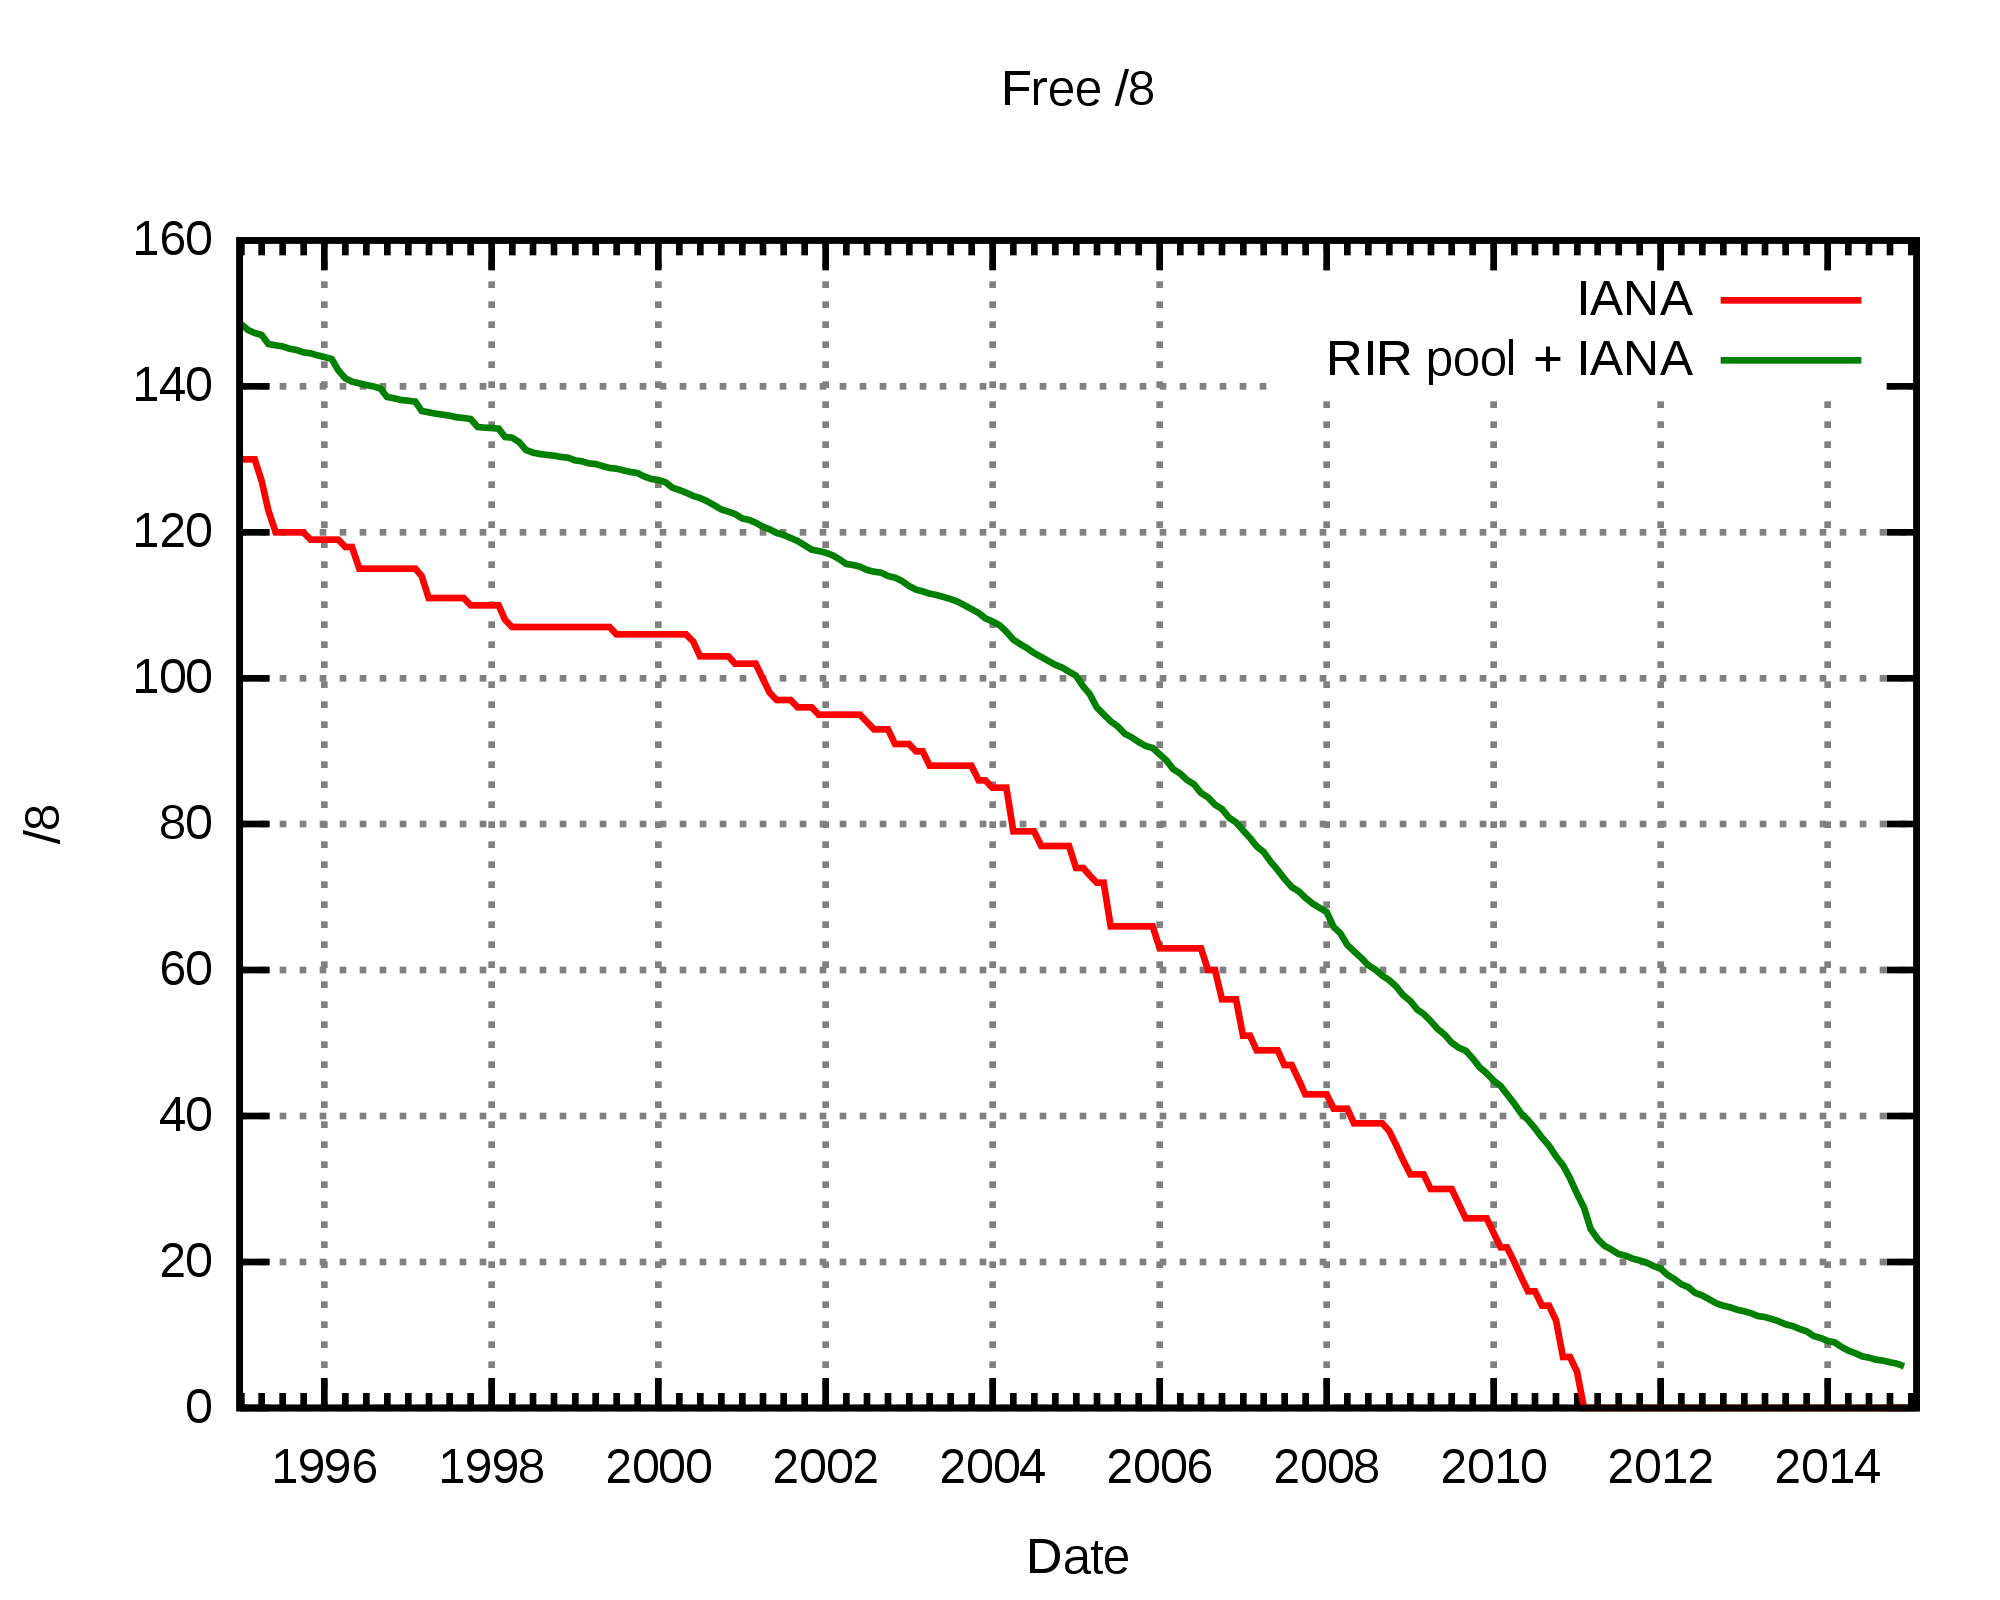
\includegraphics[width=\textwidth,keepaspectratio]{img/01}
	\source{https://upload.wikimedia.org/wikipedia/commons/c/cf/Ipv4-exhaust.svg}
	\caption{Wolne pule adresów IPv4 w czasie}
\end{figure}

Biorąc pod uwagę powyższe, na mocy Zasady Szufladkowej Dirichleta możemy
stwierdzić, że adres IPv4 nie jest już identyfikatorem, który mógłby unikatowo
identyfikować każde urządzenie podłączone do Internetu. W tym momencie warto
także zaznaczyć, że o ile nowy standard IPv6 pozwalałby na taką identyfikację,
to został on zaprojektowany z myślą o prywatności i posiada szereg rozszerzeń,
które w przyszłości (kiedy Internet w pełni przejdzie na adresację w wersji
szóstej) mają zapobiegać precyzyjnej identyfikacji \cite{narten2001privacy}.

\subsubsection{Cookies}
Małe porcje informacji zapisywane na urządzeniu użytkownika w obszarze pamięci
trwałej przeglądarki po interakcji ze stroną internetową, która je zapisuje.
Powstały głównie ze względu na potrzebę poprawienia doświadczeń użytkowników ze
stronami internetowymi tak, aby zapamiętywać pewien stan o znaczeniu dla danej
sesji dla danego użytkownika (na przykład stan koszyka w sklepie internetowym).

\emph{Cookies} dzielą się na tak zwane \emph{first-party cookies} i
\emph{third-party cookies}. O ile pierwsze z wymienionego podziału faktycznie
desygnowane są do tego, aby spełniać wymienioną funkcję, to \emph{third-party
cookies} mogą być nadawane przez (na przykład) skrypty reklamowe umieszczone na
serwującej je stronie, dzięki czemu użytkownik może być śledzony w kontekście
całej sieci reklamowej. Ubogie mechanizmy kontroli \emph{cookies} w
przeglądarkach internetowych i obawy związane z naruszaniem prywatności
użytkowników przez śledzenie wykorzystujące \emph{cookies} doprowadziły do
powstania dyrektywy Unii Europejskiej dotyczącej obowiązku informacyjnego, która
zawiera m.in. obowiązek informowania o polityce stosowania \emph{cookies}.
Doprowadziło to wcześniej także do powstania rozszerzeń w przeglądarkach, takich
jak nagłówek Do Not Track i Tryb Prywatny, które w domyśle miały pomóc częściowo
rozwiązać wspomniany problem.

Niektóre przeglądarki internetowe, takie jak Apple Safari (Intelligent Tracking
Prevention silnika WebKit) lub Mozilla Firefox, wykorzystują obecnie natywne
mechanizmy inteligentnego blokowania \emph{third-party cookies}. Powstało także
wiele rozszerzeń do przeglądarek, które pozwalają blokować niechciane
\emph{cookies}.

\subsubsection{Inne metody identyfikacji użytkowników}
\emph{Fingerprinting} urządzeń podłączonych do Internetu i przeglądarek
internetowych to jedna ze zbioru wymyślnych technik, które zaczęto stosować ze
względu na ułomność lub postępujące ograniczenia metod wykorzystujących na
przykład adresy IP urządzeń, lub \emph{cookies}. \emph{Fingerprinting}
przeglądarek po raz pierwszy opisał Eckersley jako technikę, która pozwala
serwerom WWW jednoznacznie zidentyfikować urządzenie użytkownika za pomocą
informacji wysyłanych przez przeglądarkę internetową, wtedy kiedy te informacje
są unikalne dla większości z nich, tworząc ich \emph{fingerprint}
\cite{eckersley2010unique}. Relację urządzeń i przeglądarek pomiędzy ich
użytkownikami opisuje 2.2.

\section{Fingerprinting w branży komputerowej}
\emph{Fingerprinting} to technika wykorzystywana w wielu obszarach w dyscyplinie
informatyki; \emph{fingerprinting} urządzeń podłączonych do Internetu i
przeglądarek internetowych to tylko pewien wycinek zastosowań tej koncepcji. O
ile podane na początku tego rozdziału definicje ujmują \emph{fingerprint} w
sposób ogólny i także taki, który jest spójny z definicjami, które można znaleźć
w publikacjach dotyczących \emph{fingerprintingu} urządzeń i przeglądarek, to
definicje dotyczące zastosowań \emph{fingerprintu} innych bytów mogą być
bardziej specyficzne czy też mogą eksponować inne właściwości, charakterystyczne
dla stosownych zastosowań. Kolejne punkty służą jako referencja do ukazania jak
szeroko wykorzystywana jest omawiana koncepcja.

\subsection{Fingerprinting audio, wideo i technologia ACR}
Metody \emph{fingerprintingu} akustycznego i cyfrowych materiałów wideo, znane
także jako technologia Automatic Content Recognition (ACR), zostały
zaprezentowane w 2012 podczas Consumer Electronics Show, pokazując, że
urządzenia dostępne dla zwykłego konsumenta mogą być na tyle sprytne by
wyszukiwać informacje w oparciu o kontekst \cite{ng2012brief}. Technologia ACR
sparametryzowana jest w podobny sposób, co algorytmy \emph{fingerprintingu}
urządzeń i przeglądarek, czyli istotny jest balans pomiędzy niepowtarzalnością a
stabilnością \emph{fingerprintu}. Klasyfikacja \emph{fingerprintu} audio lub
wideo musi działać w podobny sposób do zachowania ludzkiego moderatora, czyli w
przypadku kiedy materiał jest nieodróżnialny dla ludzkiego ucha lub oka jako
ten, wobec którego przeprowadzany jest proces rozpoznawania, to powinien on
zostać oflagowany. Proces wykorzystywany przez technologię Automatic Content
Recognition określany jest mianem \emph{perceptual hashing}.

\subsection{Fingerprinting klucza publicznego}
W kryptografii klucza publicznego, w celach autoryzacji klucza publicznego
pozyskanego w niezaufany sposób (na przykład ściągając go ze strony
internetowej), poprzez zaufany kanał wymiany informacji (zwykle rozmowa
telefoniczna), który nie pozwala na autoryzację całego klucza w efektywny
sposób, stosuje się jego skrót, nazywany ,,fingerprintem klucza publicznego''.
Wynik zastosowania odpowiedniej funkcji skrótu na kluczu publicznym jest na tyle
kompaktowy, że pozwala na efektywną manualną autoryzację, czyli ręcznie przez
człowieka.

W celu ułatwienia wymiany \emph{fingerprintów} kluczy publicznych poprzez kanały
głosowe powstała lista słów PGP, która analogicznie do alfabetu fonetycznego
NATO asocjuje każdą kolejną porcję bitów \emph{fingerprintu} klucza z
odpowiednim słowem w języku angielskim.

\chapter{Problematyka prywatności i anonimowości w Internecie}
Technika, o której traktuje ta praca, jest ważnym tematem głównie dlatego, że
wykorzystanie jej do identyfikacji użytkowników ma istotne implikacje w obszarze
prywatności i anonimowości.

\section{Prywatność i anonimowość}
Prywatność internetowa to pewien podzbiór relacji pomiędzy gromadzeniem i
rozpowszechnianiem danych, technologią, społecznym oczekiwaniom wobec
prywatności i prawnymi oraz politycznym problemami orbitującymi wokół tych
zagadnień \cite{michael2013uberveillance}. W celach orientacyjnych stosowanym
uproszczeniem jest pogląd, że prywatność internetowa to możliwość zatrzymania
związanych z własną aktywnością danych dla siebie. Anonimowością jest zatem
sytuacja, w której przekazywanie takich danych jest zablokowane.

Prywatność i anonimowość użytkowników Internetu stała się zagadnieniem jeszcze
przed nadejściem ery Internetu \cite{david1965some}, pozwalając na koniec lat
dziewięćdziesiątych na zaognienie dyskusji, która trwa do dzisiaj. Użytkownicy
Internetu mają różne oczekiwania wobec poziomu ich prywatności w sieci. Mniej
wyczuleni na punkcie prywatności użytkownicy są w stanie pójść na pewny
kompromis pomiędzy wykorzystaniem ich danych a oferowanym na tej podstawie
potencjalnym usprawnieniem ich doświadczeń w Internecie (na przykład na
konkretnych stronach internetowych, w kontekście sieci reklamowych lub w innych
szerszych, kontekstach). Akceptują oni ryzyko zbyt szczegółowego profilowania,
potencjalnych naruszeń prywatności i inwigilacji. Inni użytkownicy dążą (mniej
lub bardziej) do utrzymania anonimowości takiej, jaka panowała w Internecie na
początku jego istnienia \cite[s. 54--69]{snowden2019pamiec}.

\subsection{Łączenie danych}
Istnieją firmy specjalizujące się w pozyskiwaniu, kupowaniu i przetwarzaniu
danych użytkowników w różnych celach (zwykle reklamowych). Nie wszystkie firmy
rynku danych przetwarzają dane w sposób naruszający prywatność użytkowników, ale
techniki takie jak łączenie danych z różnych źródeł (bez uprzedniej
anonimizacji) mogą lub będą prowadzić do nadużyć.

Bardzo sławny przypadek firmy Cambridge Analytica, która tworzyła profile
psychologiczne użytkowników i używała ich do manipulacji opinią publiczną za
pomocą mediów społecznościowych to jeden z przykładów firmy, która łącząc dane,
poważnie naruszyła prywatność użytkowników (m.in. Facebooka).

Istnieje wiele różnych dróg, dzięki którym w Internecie i w świecie rzeczywistym
użytkownicy będą nieświadomie profilowani lub inwigilowani, a łączenie danych z
różnych źródeł istotnie poprawi dokładność obrazu użytkownika. Jedną z takich
dróg jest używanie stron internetowych będących częścią większej sieci
reklamowej, która łączy dane na przykład z portali \emph{social media}, wyników
wyszukiwań, wysyłanych formularzy, a nawet z takich źródeł jak systemów
automatycznego wykrywania twarzy w sklepach stacjonarnych. Niektóre informacje,
które można wnioskować po automatycznym przetworzeniu to orientacja seksualna,
poglądy polityczne i religijne, rasa, historia użycia substancji
psychoaktywnych, estymowany iloraz inteligencji czy osobowość
\cite{kosinski2013private}.

\subsection{Czy prywatność jest nam potrzebna?}
Ochrona prywatności ma swoich przeciwników i zwolenników. ,,nie obchodzi mnie
prywatność, bo nie mam nic do ukrycia'' to argument przytaczany przez
przeciwników ochrony prywatności. Jedną z ważnych osób, które opowiedziały się
niegdyś za taką argumentacją, jest Eric Schmidt, były CEO firmy Google. Istnieje
silna polaryzacja pomiędzy przeciwnikami i zwolennikami ochrony prywatności. W
swojej książce autobiograficznej Edward Snowden (słynny amerykański
\emph{whistleblower}) stwierdził, że ,,oświadczyć, że nie obchodzi cię
prywatność, bo nie masz nic do ukrycia, to mniej więcej to samo, co oświadczyć,
że nie obchodzi cię wolność słowa, ponieważ nie masz nic do powiedzenia''
\cite{snowden2019pamiec}. Bruce Schneier, amerykański kryptograf i ekspert w
dziedzinie bezpieczeństwa komputerowego podsumowuje, że zbyt wiele osób myśli o
tym argumencie jak o wyborze pomiędzy bezpieczeństwem a prywatnością.
,,Prawdziwym wyborem jest wybór pomiędzy wolnością a kontrolą''
\cite{schneier2006eternal}. Prawo do prywatności zawiera się w Powszechnej
Deklaracji Praw Człowieka \cite{united1949universal}.

\section{Metody identyfikacji użytkowników}
Tak ja zauważono wcześniej w niniejszej pracy---wraz z komercjalizacją Internetu
powstał i ewoluował szereg różnych metod identyfikacji urządzeń, przeglądarek i
tym samym użytkowników. Istnieją różne zastosowania identyfikacji, ale jednym z
najbardziej powszechnie omawianych (i kontrowersyjnych) jest śledzenie
użytkowników (formalnie: łączenie ze sobą wielu wizyt jednego użytkownika na tej
samej platformie) \cite[s. 3]{al2020too}.

Warto także zauważyć, że \emph{fingerprinting} przeglądarek internetowych to
jedna z dróg identyfikacji urządzeń podłączonych do Internetu. Jest ona jednak
na tyle reprezentatywna, że często mówi się o \emph{fingerprintingu} urządzeń
jako \emph{fingerprintingu} przeglądarek. Dzieje się tak, ponieważ dzisiejsze
przeglądarki internetowe podczas interakcji z serwerami WWW mogą aktywnie lub
pasywnie przekazywać zestaw danych na tyle szeroki \cite{eckersley2010unique},
że zawiera on w sobie \emph{fingerprint} urządzenia, na którym działa
przeglądarka. Przeważający ogrom aktywności użytkowników wokół ,,przeglądania''
Internetu i wiele danych ,,oferowanych'' przez przeglądarki internetowe
naturalnie sprawia, że wysiłki identyfikujące użytkowników rozważane są głównie
w kontekście tychże. Niniejsza praca stara się zapewnić pewien (choć często
niewidoczny) podział. W kolejnym rozdziale niniejszej pracy omówiony jest także
\emph{fingerprinting} urządzeń podłączonych do Internetu, kiedy niemożliwe jest
wykorzystanie do celów identyfikacyjnych przeglądarki internetowej użytkownika.

Identyfikacja użytkowników nie zawsze jest także synonimem z identyfikacją
urządzeń czy przeglądarek, ale odsetek przypadków, kiedy w dzisiejszym świecie
więcej niż jedna osoba korzysta z np. jednej przeglądarki internetowej, wydaje
się stosunkowo niski. Powodem dla takiej estymacji jest fakt, iż wspomniane
przeglądarki, które posiadają istotny ułamek udziałów w rynku przeglądarek
internetowych, posiadają mechanizmy pozwalające na ich jednoznaczną
personalizację (parowanie z personalnym kontem Google w przeglądarce Google
Chrome, integracja przeglądarki Safari z ekosystemem firmy Apple, parowanie z
personalnym kontem Firefox w przeglądarce Firefox itd.). Co więcej, jeden
użytkownik może korzystać z wielu przeglądarek, co utrudnia jednoznaczną
identyfikację, ale nie czyni jej niemożliwą. Istnieją bowiem metody
\emph{fingerprintingu} urządzeń i przeglądarek pozwalające na identyfikację
użytkowników pomiędzy przeglądarkami internetowymi zainstalowanymi na tym samym
urządzeniu.

Gdyby podsumować metody identyfikacji użytkowników w dzisiejszym Internecie to
ich niedługa lista prezentowałaby się następująco:
\begin{itemize}
	\item Użycie \emph{cookies} (w szczególności \emph{third-party cookies});
	\item Użycie \emph{supercookies};
	\item Użycie \emph{fingerprintingu}.
\end{itemize}

Oczywiście nic nie stoi na przeszkodzie, aby każda z tych metod była używana w
połączeniu z innymi.

\section{Zagrożenia związane z fingerprintingiem}
Al-Fannah i Mitchell \cite[s. 1]{al2020too} konstatują, że identyfikacja za
pomocą \emph{fingerprintingu} jest znacznie trwalsza niż ta bazująca na
\emph{cookies}, praktycznie bez możliwości kontroli przez użytkowników i
nietrywialna do wykrycia. Istnieją zatem przynajmniej trzy powody, dla których
\emph{fingerprinting} stanowi istotnie większe zagrożenie dla prywatności
użytkowników (większe niż wszystkie dotychczasowe):
\begin{itemize}
	\item Na tę chwilę nie są znane proste sposoby, aby z całkowitą pewnością
	      wykryć, że dana platforma lub strona internetowa używa
	      \emph{fingerprintingu};
	\item Użytkownicy mogą kontrolować moc śledzenia za pomocą \emph{cookies},
	      regularnie usuwając je lub całkowicie blokując. Jak zostało
	      nadmienione wcześniej, istnieją także regulacje prawne dotyczące
	      użycia \emph{cookies}. Nie ma jednak żadnych porównywalnych, równie
	      prostych do użycia technik kontroli \emph{fingerprintingu};
	\item \emph{Fingerprinting} (w przeciwieństwie do \emph{cookies}) nie polega
	      na jednej, konkretnej właściwości HTTP. \emph{Fingerprinting} bazuje
	      na wielu technologiach, aby zbierać różne informacje o właściwościach
	      i konfiguracji przeglądarki lub systemu operacyjnego. Każda z tych
	      informacji to szansa, aby zastosować \emph{fingerprinting}.
\end{itemize}

Co więcej, \emph{fingerprinting} może być użyty do tworzenia
\emph{supercookies}, czyli specjalnych \emph{cookies}, które po usunięciu mogą
zostać ponownie utworzone, jeśli ta sama przeglądarka zostanie wykryta przez
użycie \emph{fingerprintingu} \cite[s. 2]{al2020too}.

\section{Możliwości ochrony przed fingerprintingiem}
Autorzy monografii dotyczącej metod kontroli i ochrony przed
\emph{fingerprintingiem} wyróżniają dwa typy rozwiązań ochrony przed
\emph{fingerprintingiem}: możliwe do zastosowania przez użytkowników i takie,
które powinny zostać zaimplementowane przez autorów oprogramowania
\cite{al2020too}.

\subsection{Perspektywa użytkownika}
Kontrola i ochrona, którą mogą zastosować użytkownicy to wybór przeglądarki i
jej konfiguracja (np. Firefox posiada pewne ustawienia dotyczące ograniczania
\emph{fingerprintingu}---Rys. 2) lub instalacja dodatkowych rozszerzeń, które
blokują lub ograniczają \emph{fingerprinting}, blokując JavaScript, fałszując
atrybuty lub blokując przesyłanie ich zawartości. Niestety każdy z wymienionych
sposobów wiąże się obecnie z istotną degradacją jakości przeglądania Internetu.
Przy wyborze aktualnie prawdopodobnie najbardziej skupionej na prywatności
przeglądarki Tor możemy spotkać się z wieloma ostrzeżeniami. Jest to na przykład
prośba o niemaksymalizowanie okna przeglądania, aby zapobiec efektywnemu
używaniu atrybutu rozdzielczości ekranu podczas ewentualnego
\emph{fingerprintingu}. Używając wyżej wymienionych sposobów, musimy także
liczyć się z tym, że wiele stron internetowych może po prostu przestać działać.
Niektóre z rozszerzeń, chociaż często ograniczonych przez to na jak wiele
pozwalają autorzy oprogramowania, mogą paradoksalnie przyczynić się do
dokładniejszego \emph{fingerprintingu}. Omawiany \emph{fingerprintability
	paradox} nazywa sytuację, w której próby ograniczenia \emph{fingerprintingu}
nieintencjonalnie tworzą nowe źródło danych, których można użyć w trakcie
\emph{fingerprintingu}. Problem widoczny jest szczególnie, wtedy kiedy danego
rozszerzenia używa niewielu użytkowników. Niektóre z rozszerzeń mogą także
fałszować atrybuty w taki sposób, że są one bardzo rzadkie lub wręcz
nierealistyczne. Taka sytuacja sprzyja unikalnej identyfikacji. Paradoks był
szeroko omawiany w środowisku naukowym \cite{eckersley2010unique,torres2015fp}.
Autorzy monografii podkreślają też, że nie ma obecnie żadnych poważnych badań
dotyczących efektywności istniejących rozszerzeń mających zapobiegać przed
\emph{fingerprintingiem}.

\begin{figure}
	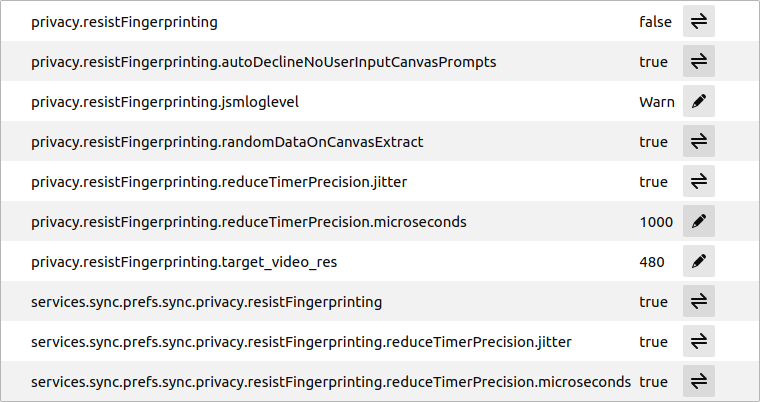
\includegraphics[width=\textwidth,keepaspectratio]{img/02}
	\source{about:config}
	\caption{Opcje ograniczające \emph{fingerprinting} w Firefox 79.0}
\end{figure}

\subsection{Perspektywa twórców oprogramowania}
Zakres działań, które mogą podjąć twórcy przeglądarek internetowych, jest
znacznie szerszy niż to, czego mogą dokonać sami użytkownicy. Aktualnie
wszystkie główne przeglądarki internetowe różnią się w stopniu dokładności
\emph{fingerprintu}, jaki może zostać utworzony na podstawie danych przez nie
dostępnych. Redukcja informacji lub całkowite wyeliminowanie niektórych
nagłówków zapytań HTTP, jednorodność w implementacji, kontekstowy dostęp i
wycofywanie starych oraz niepotrzebnych funkcji z API przeglądarek to tylko
niektóre z kroków, jakie mogłoby podjąć konsorcjum przeglądarek, aby drastycznie
zwiększyć ich prywatność. Istnieje szereg rekomendacji dotyczący tej kwestii
\cite{cooper2013privacy,doty2014fingerprinting,eckersley2010unique,nikiforakis2014workings}.
Warto także zauważyć, że praktycznie żaden z kroków możliwych do podjęcia od tej
strony nie wiąże się z utratą jakości przeglądania/funkcjonowania stron
internetowych. Niestety niektórzy producenci przeglądarek mogą być niechętni do
podejmowania kroków mających na celu ograniczyć \emph{fingerprinting}. Powodem
tej sytuacji może być fakt, że czerpią oni korzyści finansowe z serwisów
internetowych korzystających z tej metody identyfikacji \cite[s. 13]{al2020too}.

\subsection{Czy da się skutecznie zapobiec fingerprintingowi?}
Al-Fannah i Mitchell podsumowują \cite[s. 18]{al2020too}, że wydaje się
nieprawdopodobne, abyśmy w najbliższym czasie przestali słyszeć o
\emph{fingerprintingu}. Badania pokazują, że jego użycie ciągle rośnie.
Identyfikacja za pomocą \emph{fingerprintingu} ma także inne zastosowania niż
śledzenie użytkowników (patrz 2.5), więc całkowite pozbycie się go bez
zaproponowania innej alternatywy wydaje się niemożliwe do osiągnięcia w
praktyce. Jako alternatywę autorzy proponują \emph{Unique Browser Identifier}
(UBI). Sami jednak podkreślają paradoksalną naturę proponowanego rozwiązania i
obawy przed jego potencjalnie niepoprawnymi implementacjami \cite[s.
16]{al2020too}. Biorąc pod uwagę brak stanowczych kroków ze strony producentów
przeglądarek i w przypadku braku innych alternatyw przewiduje się, że efektywne
zapobieżenie \emph{fingerprintingowi} będzie w najbliższej przyszłości
niemożliwe. Mając na uwadze to, jak dużym jest zagrożeniem dla prywatności
użytkowników, bezsprzecznie jest to ważny przedmiot przyszłych badań.

\section{Inne zastosowania fingerprintingu}
Valentin Vasilyev, który zapoczątkował cieszący się dużą popularnością
otwartoźródłowy projekt
\textbf{fingerprintjs}\footnote{https://github.com/fingerprintjs/fingerprintjs2}
i jest obecnie współzałożycielem firmy
FingerprintJS\footnote{https://www.linkedin.com/in/valentin-vasilyev}, na jej
stronie internetowej\footnote{https://fingerprintjs.com} pokazuje, że
\emph{fingerprinting} posiada wiele innych, różnych zastosowań w ramach
identyfikacji użytkowników. Są to między innymi zastosowania dotyczące
wykrywania masowego i zautomatyzowanego tworzenia fałszywych kont oraz
fałszerstw (w kontekście transakcji elektronicznych) w serwisach internetowych.
Także firma Cloudflare zapobiega atakom na serwisy swoich klientów, korzystając
z techniki Google
Picasso\footnote{https://support.cloudflare.com/hc/en-us/articles/360045224651}
(\emph{fingerprinting} urządzeń i przeglądarek opracowany przez Google
\cite{45581}). \emph{Fingerprinting} może być zatem także czymś w rodzaju
drugiej warstwy uwierzytelniającej w serwisach internetowych.

\subsection{Potencjał w operacjach wojskowych w cyberprzestrzeni}

\subsubsection{Perspektywa CyberOps i InfoOps}

\chapter{Metody fingerprintingu urządzeń i przeglądarek}
Od kiedy Eckersley \cite{eckersley2010unique} po raz pierwszy opisał
\emph{fingerprinting} przeglądarek, metody \emph{fingerprintingu} zmieniały się
i ewoluowały razem z nimi. Sytuacja \emph{fingerprintingu} poszczególnych
protokołów czy implementacji stosu TCP/IP jest raczej odmienna. Choć te metody
znane są już od lat dziewięćdziesiątych (a ich implementacje to takie narzędzia
jak nmap), są relatywnie mniej ,,przebojowym'' tematem badań i eksperymentów.
Niniejszy rozdział enumeruje przez szeroką gamę metod, prezentując implementacje
najważniejszych i rozważając ich skuteczność.

\section{Pojęcie pasywnego i aktywnego fingerprintingu}
\emph{Fingerprinting} może być przeprowadzany w sposób pasywny lub aktywny.
Pasywny polega całkowicie na informacjach, do których zdobycia nie jest wymagana
interakcja z drugą stroną połączenia (np. nagłówki HTTP (takie jak
\emph{User-Agent}))---te informacje i tak zostają wysłane. Aktywny
\emph{fingerprinting} opiera się z kolei na przykład na użyciu skryptów do
wydobycia większej ilości informacji (takich jak konfiguracja przeglądarki)
\cite[s. 3]{al2020too}.

% \section{Źródła danych identyfikacyjnych urządzeń}

% \subsection{Protokoły warstwy drugiej w modelu OSI}

% \subsection{Stos TCP/IP}

% \subsubsection{Protokoły warstwy 3 i 4 w modelu OSI}

% \paragraph{IPv4}

% \paragraph{IPv6}

% \paragraph{ICMP}

% \paragraph{IEEE802.11}

% \subsection{Nierutowalne protokoły warstwy 5 (lokalny fingerprinting)}

% \subsection{Rutowalne protokoły warstwy 7}

% \section{Wybrane metody fingerprintingu urządzeń i ich systemów operacyjnych}

% \section{Przeglądarki jako specjalny przypadek fingerprintingu urządzeń}

% \section{Źródła danych identyfikacyjnych przeglądarek}

% \section{Wybrane metody fingerprintingu przeglądarek}

% \subsection{Implementacje wybranych metod fingerprintingu przeglądarek}

% \section{Implementacja przykładu identyfikacji przeglądarki}

\chapter{Eksperymentalny algorytm klasyfikatora fingerprintów}

\section{Motywacja}
Wcześniej w niniejszej pracy zostało zaznaczone, że \emph{fingerprint} może być
bardziej unikalny kosztem jego stabilności i odwrotnie. Aby zgrupować kolejne
\emph{fingerprinty} tej samej przeglądarki internetowej, których różnice
wynikają z naturalnych przemian tej przeglądarki (np. aktualizacja), możemy użyć
klasyfikatora opartego na odpowiednim algorytmie. Tę relację przedstawia Rys. 7.
Dzięki takiemu rozwiązaniu jesteśmy w stanie zachować wiarygodny wskaźnik
entropii, używając średnio bardziej unikalnych \emph{fingerprintów} o mniejszej
stabilności.

Podobne (choć bardziej ograniczone) rozwiązanie zastosował Eckersley w swojej
pracy, w której po raz pierwszy opisał \emph{fingerprinting} przeglądarek
internetowych \cite[s. 13]{eckersley2010unique}.

\begin{figure}
	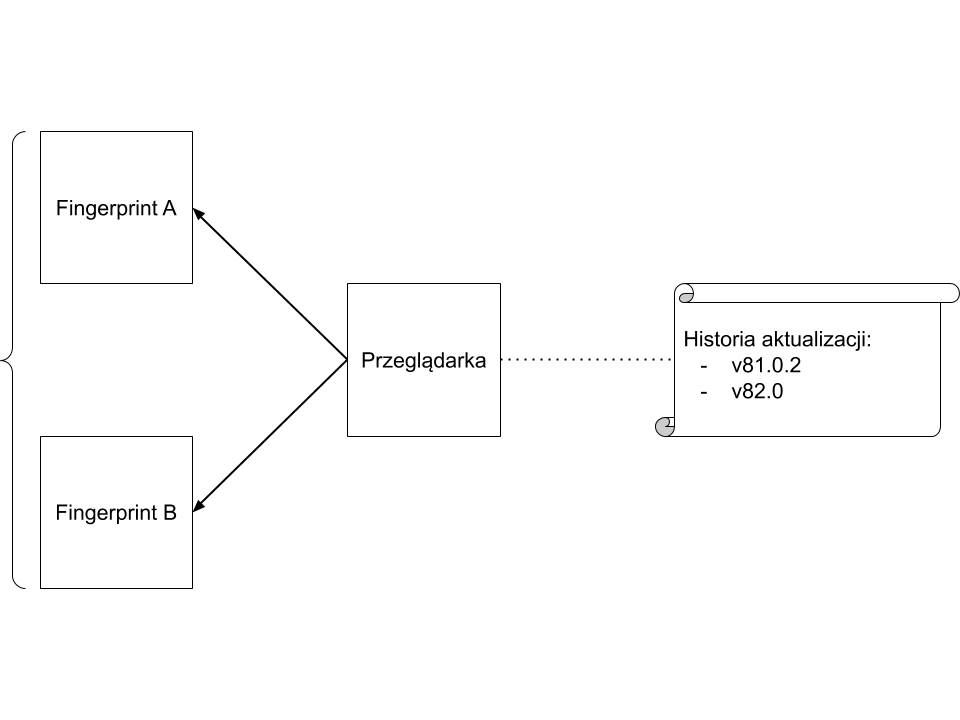
\includegraphics[width=\textwidth,keepaspectratio]{img/09}
	\source{Diagram przygotowany przez autora niniejszej pracy}
	\caption{Relacja \emph{fingerprint}--przeglądarka}
\end{figure}

\section{Opis algorytmu}
Aby zgrupować kolejne, podobne do siebie \emph{fingerprinty} należy wyznaczyć
podobieństwo każdego nowego \emph{fingerprintu} do wszystkich przechowywanych i
utożsamić go z tym, do którego jest najbardziej podobny (powyżej pewnej wartości
podobieństwa). Można to zrobić na parę sposobów. Jednym z najsensowniejszych
rozwiązań wydaje się podejście, w którym określa się podobieństwo cech
(komponentów) \emph{fingerprintu}, pomiędzy którymi istnieje relacja większości
(częściowy porządek). Tak można porównywać na przykład nagłówki User-Agent
(zawiera w sobie wersję oprogramowania) jako komponent dwóch porównywanych
\emph{fingerprintów}. Z tych porównań można wnioskować o ogólnym podobieństwie
dwóch \emph{fingerprintów}.

Porównywanie podobieństwa komponentów, które bezpośrednio lub pośrednio wynikają
z np. parametrów sprzętowych urządzenia (na przykład \emph{fingerprint} elementu
\texttt{canvas}), wydaje się bezcelowe. Ich wartość jest zwykle stała i
należałoby zastanowić się nad istnieniem częściowego porządku w takim zbiorze.
Jednakże ta niezmienność i dalej porównywanie tych komponentów na zasadzie
równoważności może być przydatne w szacowaniu, w jakim stopniu ogólne
podobieństwo jest wiarygodne.

Metryką określającą podobieństwo do siebie dwóch komponentów będzie odległość
Levenshteina, która jest powszechnie stosowaną miarą odmienności skończonych
ciągów znaków.

\subsection{Odległość Levenshteina}
Algorytmy wyznaczające odległość Levenshteina nie są na tyle popularne, aby
znalazły one swoją implementację w bibliotekach standardowych większości
popularnych języków oprogramowania. Z tego względu autor niniejszej pracy
zdecydował się na własnoręczną implementację.

\subsubsection{Definicja}
Odległość Levenshteina pomiędzy dwoma łańcuchami znaków \(a\) i \(b\) o
długościach odpowiednio \(i\) i \(j\), zdefiniowana jest jako
\begin{displaymath}
	\operatorname{ol}(i,j)=
	\begin{cases}
		\max(i,j)                    & \text{jeśli }\min(i,j)=0,  \\
		\min
		\begin{cases}
		\operatorname{ol}(i-1,j)+1 \\
		\operatorname{ol}(i,j-1)+1 \\
		\operatorname{ol}(i-1,j-1)   & \text{jeśli }a_i=b_j,      \\
		\operatorname{ol}(i-1,j-1)+1 & \text{jeśli }a_i \neq b_j. 
	\end{cases} & \text{w innym przypadku}.
	\end{cases}
\end{displaymath}

\subsubsection{Algorytm Wagnera--Fischera}
Bezpośrednia implementacja (z definicji) algorytmu wyznaczającego odległość
Levenshteina ma zasadniczy problem: tak zaimplementowany algorytm będzie działać
w czasie ponadwielomianowym. Aby się o tym przekonać, wystarczy narysować drzewo
wywołań rekurencyjnych i zauważyć, że kolejne wywołania nie są rozłączne (nie
jest to oczywiście formalny dowód). Wyznaczanie odległości Levenshteina cechuje
własność optymalnej podstruktury i bazując na programowaniu dynamicznym, można
znaleźć algorytm działający w czasie wielomianowym.

Jednym z takich algorytmów jest algorytm Wagnera--Fischera\footnote{Algorytm
	miał wielu wynalazców. Nazwa ,,Wagnera--Fischera'' powinna być traktowana
	jedynie jako zwyczajowa:
	https://en.wikipedia.org/wiki/Wagner-Fischer\_algorithm\#History} (Algorytm 2)
\cite{wagner1974string}. Implementacja 4 przedstawia implementację algorytmu
Wagnera--Fischera. Implementacja 5 jest optymalnym wariantem tego algorytmu
(biorąc pod uwagę zużycie pamięci; Implementacja 4 zużywa kwadratową ilość
pamięci a Implementacja 5 liniową). Taki wariant jest stosowany później w
algorytmie klasyfikatora.

\begin{algorithm}
	\SetAlgoVlined
	\SetAlgoCaptionSeparator{.}
	\SetKwInOut{Input}{Dane}
	\SetKwInOut{Output}{Wynik}
	\SetKwData{VarM}{m}
	\SetKwData{VarN}{n}
	\SetKwData{VarC}{c}
	\SetKwArray{VarA}{a}
	\SetKwArray{VarB}{b}
	\SetKwArray{VarD}{d}
	\SetKwArray{VarE}{}
	\SetKwFunction{Minimum}{minimum}
	\BlankLine
	\Input{ciągi znaków \VarA i \VarB o długościach odpowiednio \VarM i \VarN}
	\Output{odległość Levenshteina}
	\BlankLine
	\VarD $\leftarrow$ \VarE{$0 \dots$ \VarM, $0 \dots$ \VarN}\;
	\For{$i \leftarrow 1$ \KwTo \VarM}{
		\VarD{$i$, $0$} $\leftarrow i$\;
	}
	\For{$j \leftarrow 1$ \KwTo \VarN}{
		\VarD{$0$, $j$} $\leftarrow j$\;
	}
	\For{$j \leftarrow 1$ \KwTo \VarN}{
		\For{$i \leftarrow 1$ \KwTo \VarM}{
			\eIf{\VarA{$i - 1$} $=$ \VarB{$j - 1$}}{
				\VarC $\leftarrow 0$\;
				}{
				\VarC $\leftarrow 1$\;
			}
			\VarD{$i$, $j$} $\leftarrow$ \Minimum{\VarD{$i - 1$, $j$} $+$ $1$, \VarD{$i$, $j - 1$} $+$ $1$, \VarD{$i - 1$, $j - 1$} $+$ \VarC}\;
		}
	}
	\Return{\VarD{\VarM, \VarN}}\;
	\caption{Algorytm Wagnera--Fischera}
\end{algorithm}

\lstinputlisting[float,language=Go,caption=Algorytm Wagnera--Fischera w Go,firstline=18,lastline=44,tabsize=4]{go/levenshtein.go}

\lstinputlisting[float,language=Go,caption=Algorytm Wagnera--Fischera w Go (liniowa pamięć),firstline=46,lastline=74,tabsize=4]{go/levenshtein.go}

\section{Pseudokod}
Algorytm 3 obrazuje eksperymentalny algorytm klasyfikatora \emph{fingerprintów}.
Funkcja \texttt{hardwareRelatedCompatibility} odpowiada za binarne porównanie
wcześniej omawianych, teoretycznie niezmiennych komponentów. Funkcja
\texttt{similarity} bazując na odległości Levenshteina, przeprowadza porównanie
dla reszty komponentów. Implementacja 6 przedstawia implementację tego algorytmu
w Go.

% [ ] osCpu: getOsCpu
% [ ] languages: getLanguages
% [ ] colorDepth: getColorDepth
% [ ] deviceMemory: getDeviceMemory
% [ ] screenResolution: getScreenResolution
% [ ] availableScreenResolution: getAvailableScreenResolution
% [ ] hardwareConcurrency: getHardwareConcurrency
% [x] timezoneOffset: getTimezoneOffset
% [x] timezone: getTimezone
% [ ] sessionStorage: getSessionStorage
% [ ] localStorage: getLocalStorage
% [ ] indexedDB: getIndexedDB
% [ ] openDatabase: getOpenDatabase
% [ ] cpuClass: getCpuClass
% [?] platform: getPlatform
% [x] plugins: getPlugins
% [ ] canvas: getCanvasFingerprint
% [ ] touchSupport: getTouchSupport
% [x] fonts: getFonts
% [ ] audio: getAudioFingerprint
% [ ] pluginsSupport: getPluginsSupport
% [x] productSub: getProductSub
% [ ] emptyEvalLength: getEmptyEvalLength
% [ ] errorFF: getErrorFF
% [x] vendor: getVendor
% [ ] chrome: getChrome
% [ ] cookiesEnabled: areCookiesEnabled

\begin{algorithm}
	\SetAlgoVlined
	\SetAlgoCaptionSeparator{.}
	\SetKwInOut{Input}{Dane}
	\SetKwInOut{Output}{Wynik}
	\SetKwData{VarF}{f}
	\SetKwData{VarG}{g}
	\SetKwData{VarMax}{max}
	\SetKwData{VarRatio}{ratio}
	\SetKwData{VarCandidate}{candidate}
	\SetKwData{SetG}{G}
	\SetKwFunction{HardwareRelatedCompatibility}{hardwareRelatedCompatibility}
	\SetKwFunction{Continue}{continue}
	\SetKwFunction{Similarity}{similarity}
	\SetKw{Null}{NULL}
	\BlankLine
	\Input{Zbiór \emph{fingerprintów} \SetG i \emph{fingerprint} \VarF}
	\Output{\emph{fingerprint}, do którego \VarF jest najbardziej podobny, jeśli istnieje}
	\BlankLine
	\VarMax $\leftarrow 0$\;
	\ForEach{\VarG $\in$ \SetG}{
		\If{\HardwareRelatedCompatibility{\VarF, \VarG} $< \alpha$}{
			\Continue\;
		}
		\BlankLine
		\VarRatio $\leftarrow$ \Similarity{\VarF, \VarG}\;
		\BlankLine
		\If{\VarRatio $>$ \VarMax}{
			\VarMax $\leftarrow$ \VarRatio\;
			\VarCandidate $\leftarrow$ \VarG\;
		}
	}
	\If{\VarMax $\ge \beta$}{
		\Return{\VarCandidate}\;
	}
	\Return{\Null}\;
	\caption{Eksperymentalny klasyfikator}
\end{algorithm}

\lstinputlisting[float,language=Go,caption=Eksperymentalny klasyfikator w Go,firstline=378,lastline=401,tabsize=4]{go/classifier.go}

\section{Ocena złożoności czasowej i pamięciowej}
Załóżmy, że \texttt{hardwareRelatedCompatibility} działa w czasie stałym.
Zgodnie z wcześniejszym ustaleniami \texttt{similarity} powinna działać w czasie
co najwyżej kwadratowym, proporcjonalnym do długości \emph{fingerprintu}
(algorytm Wagnera--Fischera działa w czasie \(\Theta(mn)\), gdzie \(m\) i \(n\)
to długości porównywanych ciągów). Warto jednak zauważyć, że długość
\emph{fingerprintu} jest stała. Proponowany algorytm przegląda wszystkie
zapisane wcześniej \emph{fingerprinty} i dla każdego obrotu wykonuje stałą
pracę. Możemy zatem stwierdzić, że proponowany algorytm działa w czasie
liniowym.

Mając na uwadze rozważania z poprzedniego akapitu, możemy także stwierdzić, że
pamięć używana przez proponowany algorytm jest stała.

\section{Ocena efektywności}

\subsection{Opis utworzonego rozwiązania}

\subsection{Efektywność na przykładzie Firefox na Ubuntu}

\chapter*{Podsumowanie}
\addcontentsline{toc}{chapter}{Podsumowanie}

\section*{Fingerprinting to część dzisiejszego Internetu}
\addcontentsline{toc}{section}{Fingerprinting to część dzisiejszego Internetu}
Wszystko wskazuje na to, że \emph{fingerprinting} przeglądarek internetowych i
urządzeń podłączonych do Internetu nie odejdzie przez najbliższy czas w
niepamięć. Ta kontrowersyjna technika nie jest już jedynie trendem w gronie
metod identyfikacji użytkowników, ale wygląda na to, że stała się integralną
częścią współczesnego Internetu. Wiele firm działających w obszarze i
kształtujących Internet (w szczególności te związane z reklamą w Internecie) nie
ma w interesie ograniczania \emph{fingerprintingu} \cite{al2018beyond}.
Najpopularniejsza\footnote{https://netmarketshare.com/browser-market-share.aspx}
przeglądarka Chrome jest najprawdopodobniej najbardziej podatną \cite{al2017not}
na tę technikę przeglądarką internetową m.in. z tego powodu. Pomimo iż
specjaliści od cyberbezpieczeństwa traktują \emph{fingerprinting} nie tylko jako
lukę w zabezpieczeniach, ale także w prywatności
\cite{mowery2012pixel,al2020too}, to natychmiastowe ograniczenie go sprawi, że
część Internetu może najzwyczajniej przestać działać. Nie tylko ze względu na
to, że polega on na podstawowych funkcjonalnościach przeglądarek i ich pewnym
rozproszeniu, ale także dlatego, że niektóre serwisy polegają na
\emph{fingerprintingu} w kontekście uwierzytelniania użytkowników (na tej
zasadzie działają takie technologie jak reCAPTCHA v3) \cite{45581}. Użycie i
ochrona przed tą techniką przez służby mundurowe także zasługuje na istotną
uwagę.

\section*{Pole do usprawnień: uczenie maszynowe}
\addcontentsline{toc}{section}{Pole do usprawnień: uczenie maszynowe}
Ciągle powstają nowe metody \emph{fingerprintingu} przeglądarek i urządzeń a te
opisane w pracy stanowią jedynie fundamentalne podstawy \emph{fingerprintingu}
tychże. Są one jednak nadal skuteczne a tam, gdzie kończą się ich ,,naturalne''
możliwości identyfikacyjne mogą pomóc klasyfikatory (takie jak eksperymentalny
klasyfikator opisany w czwartym rozdziale). Proste heurystyczne algorytmy mogą
jednak okazać się wielokrotnie mniej efektywne od zastosowania metod uczenia
maszynowego do klasyfikacji \emph{fingerprintów}. Jest to wątek, którego
wykorzystanie z całą pewnością mogłoby zaowocować świetnymi wynikami.

\section*{Wnioski końcowe}
\addcontentsline{toc}{section}{Wnioski końcowe}
Idea stojąca za \emph{fingerprintingiem} jest relatywnie prosta. Mimo tego
manualne stosowanie tej idei w odniesieniu do \emph{fingerprintingu}
przeglądarek i urządzeń jest nietrywialne. Wymaga ono dobrej znajomości
ekosystemu przeglądarek, systemów operacyjnych, zależności pomiędzy różnymi
parametrami tych ekosystemów itd. Można zatem dojść do wniosku, że tworzenie
gotowych produktów jak biblioteki \emph{fingerprintingowe} (np. wspomniany
\textbf{fingerprintjs}\footnote{https://github.com/fingerprintjs/fingerprintjs2})
lub zaprezentowany eksperymentalny klasyfikator przyczynią się do skorzystania z
omawianych metod większej grupy zainteresowanych. To i opisane wcześniej
problemy są pewnymi wyzwaniami w walce o bezpieczeństwo i prywatność w
Internecie. Rozwiązania tych problemów są niestety często wielokrotnie bardziej
skomplikowane niż metody, których użycie generuje te problemy. Powyższe aspekty
składają się na wniosek, że \emph{fingerprinting} przeglądarek internetowych i
urządzeń podłączonych do Internetu jest tematem, który warto i należy dalej
zgłębiać---nie tylko przez osoby zajmujące się cyberbezpieczeństwem.

\listoffigures
\listoftables
\listofalgorithms
\lstlistoflistings
\printbibliography
\end{document}
